\documentclass[twoside]{book}

% Packages required by doxygen
\usepackage{fixltx2e}
\usepackage{calc}
\usepackage{doxygen}
\usepackage[export]{adjustbox} % also loads graphicx
\usepackage{graphicx}
\usepackage[utf8]{inputenc}
\usepackage{makeidx}
\usepackage{multicol}
\usepackage{multirow}
\PassOptionsToPackage{warn}{textcomp}
\usepackage{textcomp}
\usepackage[nointegrals]{wasysym}
\usepackage[table]{xcolor}

% Font selection
\usepackage[T1]{fontenc}
\usepackage[scaled=.90]{helvet}
\usepackage{courier}
\usepackage{amssymb}
\usepackage{sectsty}
\renewcommand{\familydefault}{\sfdefault}
\allsectionsfont{%
  \fontseries{bc}\selectfont%
  \color{darkgray}%
}
\renewcommand{\DoxyLabelFont}{%
  \fontseries{bc}\selectfont%
  \color{darkgray}%
}
\newcommand{\+}{\discretionary{\mbox{\scriptsize$\hookleftarrow$}}{}{}}

% Page & text layout
\usepackage{geometry}
\geometry{%
  a4paper,%
  top=2.5cm,%
  bottom=2.5cm,%
  left=2.5cm,%
  right=2.5cm%
}
\tolerance=750
\hfuzz=15pt
\hbadness=750
\setlength{\emergencystretch}{15pt}
\setlength{\parindent}{0cm}
\setlength{\parskip}{3ex plus 2ex minus 2ex}
\makeatletter
\renewcommand{\paragraph}{%
  \@startsection{paragraph}{4}{0ex}{-1.0ex}{1.0ex}{%
    \normalfont\normalsize\bfseries\SS@parafont%
  }%
}
\renewcommand{\subparagraph}{%
  \@startsection{subparagraph}{5}{0ex}{-1.0ex}{1.0ex}{%
    \normalfont\normalsize\bfseries\SS@subparafont%
  }%
}
\makeatother

% Headers & footers
\usepackage{fancyhdr}
\pagestyle{fancyplain}
\fancyhead[LE]{\fancyplain{}{\bfseries\thepage}}
\fancyhead[CE]{\fancyplain{}{}}
\fancyhead[RE]{\fancyplain{}{\bfseries\leftmark}}
\fancyhead[LO]{\fancyplain{}{\bfseries\rightmark}}
\fancyhead[CO]{\fancyplain{}{}}
\fancyhead[RO]{\fancyplain{}{\bfseries\thepage}}
\fancyfoot[LE]{\fancyplain{}{}}
\fancyfoot[CE]{\fancyplain{}{}}
\fancyfoot[RE]{\fancyplain{}{\bfseries\scriptsize Generated by Doxygen }}
\fancyfoot[LO]{\fancyplain{}{\bfseries\scriptsize Generated by Doxygen }}
\fancyfoot[CO]{\fancyplain{}{}}
\fancyfoot[RO]{\fancyplain{}{}}
\renewcommand{\footrulewidth}{0.4pt}
\renewcommand{\chaptermark}[1]{%
  \markboth{#1}{}%
}
\renewcommand{\sectionmark}[1]{%
  \markright{\thesection\ #1}%
}

% Indices & bibliography
\usepackage{natbib}
\usepackage[titles]{tocloft}
\setcounter{tocdepth}{3}
\setcounter{secnumdepth}{5}
\makeindex

% Hyperlinks (required, but should be loaded last)
\usepackage{ifpdf}
\ifpdf
  \usepackage[pdftex,pagebackref=true]{hyperref}
\else
  \usepackage[ps2pdf,pagebackref=true]{hyperref}
\fi
\hypersetup{%
  colorlinks=true,%
  linkcolor=blue,%
  citecolor=blue,%
  unicode%
}

% Custom commands
\newcommand{\clearemptydoublepage}{%
  \newpage{\pagestyle{empty}\cleardoublepage}%
}

\usepackage{caption}
\captionsetup{labelsep=space,justification=centering,font={bf},singlelinecheck=off,skip=4pt,position=top}

%===== C O N T E N T S =====

\begin{document}

% Titlepage & ToC
\hypersetup{pageanchor=false,
             bookmarksnumbered=true,
             pdfencoding=unicode
            }
\pagenumbering{roman}
\begin{titlepage}
\vspace*{7cm}
\begin{center}%
{\Large Starling\+\_\+\+Simulation }\\
\vspace*{1cm}
{\large Generated by Doxygen 1.8.11}\\
\end{center}
\end{titlepage}
\clearemptydoublepage
\tableofcontents
\clearemptydoublepage
\pagenumbering{arabic}
\hypersetup{pageanchor=true}

%--- Begin generated contents ---
\chapter{R\+E\+A\+D\+ME}
\label{md_src_README}
\hypertarget{md_src_README}{}
g++ -\/std=c++11 -\/o a a.\+cpp -\/l\+GL -\/l\+G\+LU -\/lglut g++ -\/std=c++11 -\/o b b.\+cpp -\/l\+GL -\/l\+G\+LU -\/lglut g++ -\/std=c++11 -\/o cube cube.\+cpp -\/l\+GL -\/l\+G\+LU -\/lglut 
\chapter{File Index}
\section{File List}
Here is a list of all files with brief descriptions\+:\begin{DoxyCompactList}
\item\contentsline{section}{src/\hyperlink{starlings_8cpp}{starlings.\+cpp} }{\pageref{starlings_8cpp}}{}
\end{DoxyCompactList}

\chapter{File Documentation}
\hypertarget{_r_e_a_d_m_e_8md}{}\section{src/\+R\+E\+A\+D\+ME.md File Reference}
\label{_r_e_a_d_m_e_8md}\index{src/\+R\+E\+A\+D\+M\+E.\+md@{src/\+R\+E\+A\+D\+M\+E.\+md}}

\hypertarget{starlings_8cpp}{}\section{src/starlings.cpp File Reference}
\label{starlings_8cpp}\index{src/starlings.\+cpp@{src/starlings.\+cpp}}
{\ttfamily \#include $<$bits/stdc++.\+h$>$}\\*
{\ttfamily \#include $<$G\+L/glut.\+h$>$}\\*
{\ttfamily \#include $<$stdio.\+h$>$}\\*
{\ttfamily \#include $<$stdlib.\+h$>$}\\*
{\ttfamily \#include $<$time.\+h$>$}\\*
{\ttfamily \#include $<$cstring$>$}\\*
{\ttfamily \#include $<$string$>$}\\*
Include dependency graph for starlings.\+cpp\+:
\nopagebreak
\begin{figure}[H]
\begin{center}
\leavevmode
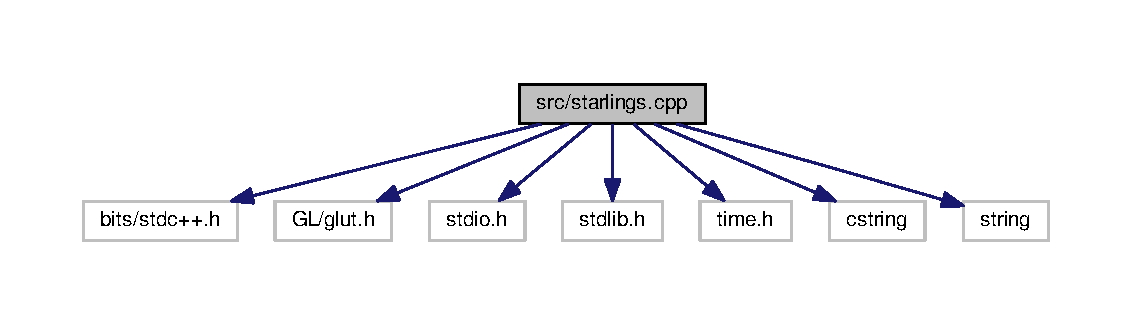
\includegraphics[width=350pt]{starlings_8cpp__incl}
\end{center}
\end{figure}
\subsection*{Functions}
\begin{DoxyCompactItemize}
\item 
void \hyperlink{starlings_8cpp_a559f65839b6a67e60dd46669b5712ab6}{wait} (float seconds)
\item 
void \hyperlink{starlings_8cpp_a7c09c503a370ef201bb27853f1cd3142}{print} (int x, int y, int z, char $\ast$string)
\item 
void \hyperlink{starlings_8cpp_ad0d8c241f9f8e69477520d2487878ff5}{add\+\_\+bird} ()
\item 
void \hyperlink{starlings_8cpp_a61a8f1d45aa146d60f7f7b8113ea2bba}{boundary} ()
\item 
void \hyperlink{starlings_8cpp_a0a30784b0a7c4911d264fccd44ae45dc}{attraction} ()
\item 
void \hyperlink{starlings_8cpp_aa59bf8641e194c92afa83a43eafd8215}{repulsion} ()
\item 
void \hyperlink{starlings_8cpp_abde5d9228861bff9b180983d32efa7f4}{update\+\_\+vel} ()
\item 
void \hyperlink{starlings_8cpp_abc2f6086b45e84f90853d92e86926836}{update\+\_\+pos} ()
\item 
void \hyperlink{starlings_8cpp_ac5c54df7ed3b930268c8d7752c101725}{update} ()
\item 
void \hyperlink{starlings_8cpp_afa20485a295d6e55ffe9d5c496d1cfa1}{idle\+\_\+fn} ()
\item 
void \hyperlink{starlings_8cpp_a2858154e2009b0e6e616f313177762bc}{init} (void)
\item 
void \hyperlink{starlings_8cpp_a4ea013001a5fb47853d0fab8f8de35cd}{display} (void)
\item 
void \hyperlink{starlings_8cpp_afd48a038baa9083e9ec15859715198ee}{animation} (void)
\item 
void \hyperlink{starlings_8cpp_a9c6a000bb585e5a23a3d829dae9d1358}{reshape} (int x, int y)
\item 
void \hyperlink{starlings_8cpp_a1564b834688cdbb8c5b7614900ce833e}{Special\+\_\+\+Keys} (int key, int x, int y)
\item 
int \hyperlink{starlings_8cpp_a3c04138a5bfe5d72780bb7e82a18e627}{main} (int argc, char $\ast$$\ast$argv)
\end{DoxyCompactItemize}
\subsection*{Variables}
\begin{DoxyCompactItemize}
\item 
G\+Lfloat \hyperlink{starlings_8cpp_a0f7dd94751a716388139167198af6f99}{x\+Rotated}
\item 
G\+Lfloat \hyperlink{starlings_8cpp_af83a51abeb599a6dd5aa9087ebc44b2a}{y\+Rotated}
\item 
G\+Lfloat \hyperlink{starlings_8cpp_ac5e754bd7fabf281ebfdb96912f69b1f}{z\+Rotated}
\item 
float \hyperlink{starlings_8cpp_aa6ea9b07932df851a61fa72bd01761fe}{size} = 0.\+02f
\item 
float \hyperlink{starlings_8cpp_ab9391faa6d1c5e72b1895547e4ef6a00}{limit} = 1.\+0f
\item 
map$<$ int, map$<$ string, float $>$ $>$ \hyperlink{starlings_8cpp_a7fb0384d64964bdc05225adfa0594e89}{position}
\item 
map$<$ int, float $>$ \hyperlink{starlings_8cpp_acd11b4fca2cf4313de76e94fcd3439bd}{vel1}
\item 
map$<$ int, float $>$ \hyperlink{starlings_8cpp_afa817b638ca7fbdae24eb2d32789a26a}{vel2}
\item 
map$<$ int, float $>$ \hyperlink{starlings_8cpp_a86b5e9d70d2601237f63e6f89c98eba7}{vel3}
\item 
float \hyperlink{starlings_8cpp_a2600896dfdf08a685fe4272f14c10b52}{axis\+\_\+size} = 2.\+0f
\item 
float \hyperlink{starlings_8cpp_ac484ca7bc54173e1bb895fa813b8a8dd}{rel\+\_\+dist} = 0.\+1f
\item 
float \hyperlink{starlings_8cpp_af4e7f730dd365cf7a28b46888a917ca2}{sumx} =0.\+0
\item 
float \hyperlink{starlings_8cpp_a14ad0bac674463aa74565ee55fa82268}{sumy} =0.\+0
\item 
float \hyperlink{starlings_8cpp_a548210e3a99d838187e42369af14aeb0}{sumz} =0.\+0
\item 
float \hyperlink{starlings_8cpp_a32e90c8902fd0c39d8387e9fe45224cd}{sumv1} =0.\+0
\item 
float \hyperlink{starlings_8cpp_a01338e4d61070945e4dfa51df9f894b5}{sumv2} =0.\+0
\item 
float \hyperlink{starlings_8cpp_a6ed82249badbcab82929c0b2210e546f}{sumv3} =0.\+0
\item 
float \hyperlink{starlings_8cpp_a0ae25983db419f389b475cf8918b0676}{suma1} =0.\+0
\item 
float \hyperlink{starlings_8cpp_a44b28585653a41346fc759066c703298}{suma2} =0.\+0
\item 
float \hyperlink{starlings_8cpp_a31cf315160e72e8cdfd612f241f3661d}{suma3} =0.\+0
\item 
float \hyperlink{starlings_8cpp_ad0952eff2667e5af2b307ba4f6d0b06b}{force} =0.\+0
\item 
float \hyperlink{starlings_8cpp_a28342d60f96d731271cfa20c110be44e}{rad} =3.\+0f
\item 
float \hyperlink{starlings_8cpp_aaa18bd78bd58de6bfe145d49f9715c01}{vr} = 1.\+0
\item 
float \hyperlink{starlings_8cpp_a2d107b3b2dcebab8a10c9d39894f6b2a}{energy} = 0.\+0f
\item 
int \hyperlink{starlings_8cpp_a76f11d9a0a47b94f72c2d0e77fb32240}{n} = 0
\end{DoxyCompactItemize}


\subsection{Function Documentation}
\index{starlings.\+cpp@{starlings.\+cpp}!add\+\_\+bird@{add\+\_\+bird}}
\index{add\+\_\+bird@{add\+\_\+bird}!starlings.\+cpp@{starlings.\+cpp}}
\subsubsection[{\texorpdfstring{add\+\_\+bird()}{add_bird()}}]{\setlength{\rightskip}{0pt plus 5cm}void add\+\_\+bird (
\begin{DoxyParamCaption}
{}
\end{DoxyParamCaption}
)}\hypertarget{starlings_8cpp_ad0d8c241f9f8e69477520d2487878ff5}{}\label{starlings_8cpp_ad0d8c241f9f8e69477520d2487878ff5}
\index{starlings.\+cpp@{starlings.\+cpp}!animation@{animation}}
\index{animation@{animation}!starlings.\+cpp@{starlings.\+cpp}}
\subsubsection[{\texorpdfstring{animation(void)}{animation(void)}}]{\setlength{\rightskip}{0pt plus 5cm}void animation (
\begin{DoxyParamCaption}
\item[{void}]{}
\end{DoxyParamCaption}
)}\hypertarget{starlings_8cpp_afd48a038baa9083e9ec15859715198ee}{}\label{starlings_8cpp_afd48a038baa9083e9ec15859715198ee}
\index{starlings.\+cpp@{starlings.\+cpp}!attraction@{attraction}}
\index{attraction@{attraction}!starlings.\+cpp@{starlings.\+cpp}}
\subsubsection[{\texorpdfstring{attraction()}{attraction()}}]{\setlength{\rightskip}{0pt plus 5cm}void attraction (
\begin{DoxyParamCaption}
{}
\end{DoxyParamCaption}
)}\hypertarget{starlings_8cpp_a0a30784b0a7c4911d264fccd44ae45dc}{}\label{starlings_8cpp_a0a30784b0a7c4911d264fccd44ae45dc}
\index{starlings.\+cpp@{starlings.\+cpp}!boundary@{boundary}}
\index{boundary@{boundary}!starlings.\+cpp@{starlings.\+cpp}}
\subsubsection[{\texorpdfstring{boundary()}{boundary()}}]{\setlength{\rightskip}{0pt plus 5cm}void boundary (
\begin{DoxyParamCaption}
{}
\end{DoxyParamCaption}
)}\hypertarget{starlings_8cpp_a61a8f1d45aa146d60f7f7b8113ea2bba}{}\label{starlings_8cpp_a61a8f1d45aa146d60f7f7b8113ea2bba}
\index{starlings.\+cpp@{starlings.\+cpp}!display@{display}}
\index{display@{display}!starlings.\+cpp@{starlings.\+cpp}}
\subsubsection[{\texorpdfstring{display(void)}{display(void)}}]{\setlength{\rightskip}{0pt plus 5cm}void display (
\begin{DoxyParamCaption}
\item[{void}]{}
\end{DoxyParamCaption}
)}\hypertarget{starlings_8cpp_a4ea013001a5fb47853d0fab8f8de35cd}{}\label{starlings_8cpp_a4ea013001a5fb47853d0fab8f8de35cd}
\index{starlings.\+cpp@{starlings.\+cpp}!idle\+\_\+fn@{idle\+\_\+fn}}
\index{idle\+\_\+fn@{idle\+\_\+fn}!starlings.\+cpp@{starlings.\+cpp}}
\subsubsection[{\texorpdfstring{idle\+\_\+fn()}{idle_fn()}}]{\setlength{\rightskip}{0pt plus 5cm}void idle\+\_\+fn (
\begin{DoxyParamCaption}
{}
\end{DoxyParamCaption}
)}\hypertarget{starlings_8cpp_afa20485a295d6e55ffe9d5c496d1cfa1}{}\label{starlings_8cpp_afa20485a295d6e55ffe9d5c496d1cfa1}
\index{starlings.\+cpp@{starlings.\+cpp}!init@{init}}
\index{init@{init}!starlings.\+cpp@{starlings.\+cpp}}
\subsubsection[{\texorpdfstring{init(void)}{init(void)}}]{\setlength{\rightskip}{0pt plus 5cm}void init (
\begin{DoxyParamCaption}
\item[{void}]{}
\end{DoxyParamCaption}
)}\hypertarget{starlings_8cpp_a2858154e2009b0e6e616f313177762bc}{}\label{starlings_8cpp_a2858154e2009b0e6e616f313177762bc}
\index{starlings.\+cpp@{starlings.\+cpp}!main@{main}}
\index{main@{main}!starlings.\+cpp@{starlings.\+cpp}}
\subsubsection[{\texorpdfstring{main(int argc, char $\ast$$\ast$argv)}{main(int argc, char **argv)}}]{\setlength{\rightskip}{0pt plus 5cm}int main (
\begin{DoxyParamCaption}
\item[{int}]{argc, }
\item[{char $\ast$$\ast$}]{argv}
\end{DoxyParamCaption}
)}\hypertarget{starlings_8cpp_a3c04138a5bfe5d72780bb7e82a18e627}{}\label{starlings_8cpp_a3c04138a5bfe5d72780bb7e82a18e627}
\index{starlings.\+cpp@{starlings.\+cpp}!print@{print}}
\index{print@{print}!starlings.\+cpp@{starlings.\+cpp}}
\subsubsection[{\texorpdfstring{print(int x, int y, int z, char $\ast$string)}{print(int x, int y, int z, char *string)}}]{\setlength{\rightskip}{0pt plus 5cm}void print (
\begin{DoxyParamCaption}
\item[{int}]{x, }
\item[{int}]{y, }
\item[{int}]{z, }
\item[{char $\ast$}]{string}
\end{DoxyParamCaption}
)}\hypertarget{starlings_8cpp_a7c09c503a370ef201bb27853f1cd3142}{}\label{starlings_8cpp_a7c09c503a370ef201bb27853f1cd3142}
\index{starlings.\+cpp@{starlings.\+cpp}!repulsion@{repulsion}}
\index{repulsion@{repulsion}!starlings.\+cpp@{starlings.\+cpp}}
\subsubsection[{\texorpdfstring{repulsion()}{repulsion()}}]{\setlength{\rightskip}{0pt plus 5cm}void repulsion (
\begin{DoxyParamCaption}
{}
\end{DoxyParamCaption}
)}\hypertarget{starlings_8cpp_aa59bf8641e194c92afa83a43eafd8215}{}\label{starlings_8cpp_aa59bf8641e194c92afa83a43eafd8215}
\index{starlings.\+cpp@{starlings.\+cpp}!reshape@{reshape}}
\index{reshape@{reshape}!starlings.\+cpp@{starlings.\+cpp}}
\subsubsection[{\texorpdfstring{reshape(int x, int y)}{reshape(int x, int y)}}]{\setlength{\rightskip}{0pt plus 5cm}void reshape (
\begin{DoxyParamCaption}
\item[{int}]{x, }
\item[{int}]{y}
\end{DoxyParamCaption}
)}\hypertarget{starlings_8cpp_a9c6a000bb585e5a23a3d829dae9d1358}{}\label{starlings_8cpp_a9c6a000bb585e5a23a3d829dae9d1358}
\index{starlings.\+cpp@{starlings.\+cpp}!Special\+\_\+\+Keys@{Special\+\_\+\+Keys}}
\index{Special\+\_\+\+Keys@{Special\+\_\+\+Keys}!starlings.\+cpp@{starlings.\+cpp}}
\subsubsection[{\texorpdfstring{Special\+\_\+\+Keys(int key, int x, int y)}{Special_Keys(int key, int x, int y)}}]{\setlength{\rightskip}{0pt plus 5cm}void Special\+\_\+\+Keys (
\begin{DoxyParamCaption}
\item[{int}]{key, }
\item[{int}]{x, }
\item[{int}]{y}
\end{DoxyParamCaption}
)}\hypertarget{starlings_8cpp_a1564b834688cdbb8c5b7614900ce833e}{}\label{starlings_8cpp_a1564b834688cdbb8c5b7614900ce833e}
\index{starlings.\+cpp@{starlings.\+cpp}!update@{update}}
\index{update@{update}!starlings.\+cpp@{starlings.\+cpp}}
\subsubsection[{\texorpdfstring{update()}{update()}}]{\setlength{\rightskip}{0pt plus 5cm}void update (
\begin{DoxyParamCaption}
{}
\end{DoxyParamCaption}
)}\hypertarget{starlings_8cpp_ac5c54df7ed3b930268c8d7752c101725}{}\label{starlings_8cpp_ac5c54df7ed3b930268c8d7752c101725}
\index{starlings.\+cpp@{starlings.\+cpp}!update\+\_\+pos@{update\+\_\+pos}}
\index{update\+\_\+pos@{update\+\_\+pos}!starlings.\+cpp@{starlings.\+cpp}}
\subsubsection[{\texorpdfstring{update\+\_\+pos()}{update_pos()}}]{\setlength{\rightskip}{0pt plus 5cm}void update\+\_\+pos (
\begin{DoxyParamCaption}
{}
\end{DoxyParamCaption}
)}\hypertarget{starlings_8cpp_abc2f6086b45e84f90853d92e86926836}{}\label{starlings_8cpp_abc2f6086b45e84f90853d92e86926836}
\index{starlings.\+cpp@{starlings.\+cpp}!update\+\_\+vel@{update\+\_\+vel}}
\index{update\+\_\+vel@{update\+\_\+vel}!starlings.\+cpp@{starlings.\+cpp}}
\subsubsection[{\texorpdfstring{update\+\_\+vel()}{update_vel()}}]{\setlength{\rightskip}{0pt plus 5cm}void update\+\_\+vel (
\begin{DoxyParamCaption}
{}
\end{DoxyParamCaption}
)}\hypertarget{starlings_8cpp_abde5d9228861bff9b180983d32efa7f4}{}\label{starlings_8cpp_abde5d9228861bff9b180983d32efa7f4}
\index{starlings.\+cpp@{starlings.\+cpp}!wait@{wait}}
\index{wait@{wait}!starlings.\+cpp@{starlings.\+cpp}}
\subsubsection[{\texorpdfstring{wait(float seconds)}{wait(float seconds)}}]{\setlength{\rightskip}{0pt plus 5cm}void wait (
\begin{DoxyParamCaption}
\item[{float}]{seconds}
\end{DoxyParamCaption}
)}\hypertarget{starlings_8cpp_a559f65839b6a67e60dd46669b5712ab6}{}\label{starlings_8cpp_a559f65839b6a67e60dd46669b5712ab6}


\subsection{Variable Documentation}
\index{starlings.\+cpp@{starlings.\+cpp}!axis\+\_\+size@{axis\+\_\+size}}
\index{axis\+\_\+size@{axis\+\_\+size}!starlings.\+cpp@{starlings.\+cpp}}
\subsubsection[{\texorpdfstring{axis\+\_\+size}{axis_size}}]{\setlength{\rightskip}{0pt plus 5cm}float axis\+\_\+size = 2.\+0f}\hypertarget{starlings_8cpp_a2600896dfdf08a685fe4272f14c10b52}{}\label{starlings_8cpp_a2600896dfdf08a685fe4272f14c10b52}
\index{starlings.\+cpp@{starlings.\+cpp}!energy@{energy}}
\index{energy@{energy}!starlings.\+cpp@{starlings.\+cpp}}
\subsubsection[{\texorpdfstring{energy}{energy}}]{\setlength{\rightskip}{0pt plus 5cm}float energy = 0.\+0f}\hypertarget{starlings_8cpp_a2d107b3b2dcebab8a10c9d39894f6b2a}{}\label{starlings_8cpp_a2d107b3b2dcebab8a10c9d39894f6b2a}
\index{starlings.\+cpp@{starlings.\+cpp}!force@{force}}
\index{force@{force}!starlings.\+cpp@{starlings.\+cpp}}
\subsubsection[{\texorpdfstring{force}{force}}]{\setlength{\rightskip}{0pt plus 5cm}float force =0.\+0}\hypertarget{starlings_8cpp_ad0952eff2667e5af2b307ba4f6d0b06b}{}\label{starlings_8cpp_ad0952eff2667e5af2b307ba4f6d0b06b}
\index{starlings.\+cpp@{starlings.\+cpp}!limit@{limit}}
\index{limit@{limit}!starlings.\+cpp@{starlings.\+cpp}}
\subsubsection[{\texorpdfstring{limit}{limit}}]{\setlength{\rightskip}{0pt plus 5cm}float limit = 1.\+0f}\hypertarget{starlings_8cpp_ab9391faa6d1c5e72b1895547e4ef6a00}{}\label{starlings_8cpp_ab9391faa6d1c5e72b1895547e4ef6a00}
\index{starlings.\+cpp@{starlings.\+cpp}!n@{n}}
\index{n@{n}!starlings.\+cpp@{starlings.\+cpp}}
\subsubsection[{\texorpdfstring{n}{n}}]{\setlength{\rightskip}{0pt plus 5cm}int n = 0}\hypertarget{starlings_8cpp_a76f11d9a0a47b94f72c2d0e77fb32240}{}\label{starlings_8cpp_a76f11d9a0a47b94f72c2d0e77fb32240}
\index{starlings.\+cpp@{starlings.\+cpp}!position@{position}}
\index{position@{position}!starlings.\+cpp@{starlings.\+cpp}}
\subsubsection[{\texorpdfstring{position}{position}}]{\setlength{\rightskip}{0pt plus 5cm}map$<$int, map$<$string,float$>$ $>$ position}\hypertarget{starlings_8cpp_a7fb0384d64964bdc05225adfa0594e89}{}\label{starlings_8cpp_a7fb0384d64964bdc05225adfa0594e89}
\index{starlings.\+cpp@{starlings.\+cpp}!rad@{rad}}
\index{rad@{rad}!starlings.\+cpp@{starlings.\+cpp}}
\subsubsection[{\texorpdfstring{rad}{rad}}]{\setlength{\rightskip}{0pt plus 5cm}float rad =3.\+0f}\hypertarget{starlings_8cpp_a28342d60f96d731271cfa20c110be44e}{}\label{starlings_8cpp_a28342d60f96d731271cfa20c110be44e}
\index{starlings.\+cpp@{starlings.\+cpp}!rel\+\_\+dist@{rel\+\_\+dist}}
\index{rel\+\_\+dist@{rel\+\_\+dist}!starlings.\+cpp@{starlings.\+cpp}}
\subsubsection[{\texorpdfstring{rel\+\_\+dist}{rel_dist}}]{\setlength{\rightskip}{0pt plus 5cm}float rel\+\_\+dist = 0.\+1f}\hypertarget{starlings_8cpp_ac484ca7bc54173e1bb895fa813b8a8dd}{}\label{starlings_8cpp_ac484ca7bc54173e1bb895fa813b8a8dd}
\index{starlings.\+cpp@{starlings.\+cpp}!size@{size}}
\index{size@{size}!starlings.\+cpp@{starlings.\+cpp}}
\subsubsection[{\texorpdfstring{size}{size}}]{\setlength{\rightskip}{0pt plus 5cm}float size = 0.\+02f}\hypertarget{starlings_8cpp_aa6ea9b07932df851a61fa72bd01761fe}{}\label{starlings_8cpp_aa6ea9b07932df851a61fa72bd01761fe}
\index{starlings.\+cpp@{starlings.\+cpp}!suma1@{suma1}}
\index{suma1@{suma1}!starlings.\+cpp@{starlings.\+cpp}}
\subsubsection[{\texorpdfstring{suma1}{suma1}}]{\setlength{\rightskip}{0pt plus 5cm}float suma1 =0.\+0}\hypertarget{starlings_8cpp_a0ae25983db419f389b475cf8918b0676}{}\label{starlings_8cpp_a0ae25983db419f389b475cf8918b0676}
\index{starlings.\+cpp@{starlings.\+cpp}!suma2@{suma2}}
\index{suma2@{suma2}!starlings.\+cpp@{starlings.\+cpp}}
\subsubsection[{\texorpdfstring{suma2}{suma2}}]{\setlength{\rightskip}{0pt plus 5cm}float suma2 =0.\+0}\hypertarget{starlings_8cpp_a44b28585653a41346fc759066c703298}{}\label{starlings_8cpp_a44b28585653a41346fc759066c703298}
\index{starlings.\+cpp@{starlings.\+cpp}!suma3@{suma3}}
\index{suma3@{suma3}!starlings.\+cpp@{starlings.\+cpp}}
\subsubsection[{\texorpdfstring{suma3}{suma3}}]{\setlength{\rightskip}{0pt plus 5cm}float suma3 =0.\+0}\hypertarget{starlings_8cpp_a31cf315160e72e8cdfd612f241f3661d}{}\label{starlings_8cpp_a31cf315160e72e8cdfd612f241f3661d}
\index{starlings.\+cpp@{starlings.\+cpp}!sumv1@{sumv1}}
\index{sumv1@{sumv1}!starlings.\+cpp@{starlings.\+cpp}}
\subsubsection[{\texorpdfstring{sumv1}{sumv1}}]{\setlength{\rightskip}{0pt plus 5cm}float sumv1 =0.\+0}\hypertarget{starlings_8cpp_a32e90c8902fd0c39d8387e9fe45224cd}{}\label{starlings_8cpp_a32e90c8902fd0c39d8387e9fe45224cd}
\index{starlings.\+cpp@{starlings.\+cpp}!sumv2@{sumv2}}
\index{sumv2@{sumv2}!starlings.\+cpp@{starlings.\+cpp}}
\subsubsection[{\texorpdfstring{sumv2}{sumv2}}]{\setlength{\rightskip}{0pt plus 5cm}float sumv2 =0.\+0}\hypertarget{starlings_8cpp_a01338e4d61070945e4dfa51df9f894b5}{}\label{starlings_8cpp_a01338e4d61070945e4dfa51df9f894b5}
\index{starlings.\+cpp@{starlings.\+cpp}!sumv3@{sumv3}}
\index{sumv3@{sumv3}!starlings.\+cpp@{starlings.\+cpp}}
\subsubsection[{\texorpdfstring{sumv3}{sumv3}}]{\setlength{\rightskip}{0pt plus 5cm}float sumv3 =0.\+0}\hypertarget{starlings_8cpp_a6ed82249badbcab82929c0b2210e546f}{}\label{starlings_8cpp_a6ed82249badbcab82929c0b2210e546f}
\index{starlings.\+cpp@{starlings.\+cpp}!sumx@{sumx}}
\index{sumx@{sumx}!starlings.\+cpp@{starlings.\+cpp}}
\subsubsection[{\texorpdfstring{sumx}{sumx}}]{\setlength{\rightskip}{0pt plus 5cm}float sumx =0.\+0}\hypertarget{starlings_8cpp_af4e7f730dd365cf7a28b46888a917ca2}{}\label{starlings_8cpp_af4e7f730dd365cf7a28b46888a917ca2}
\index{starlings.\+cpp@{starlings.\+cpp}!sumy@{sumy}}
\index{sumy@{sumy}!starlings.\+cpp@{starlings.\+cpp}}
\subsubsection[{\texorpdfstring{sumy}{sumy}}]{\setlength{\rightskip}{0pt plus 5cm}float sumy =0.\+0}\hypertarget{starlings_8cpp_a14ad0bac674463aa74565ee55fa82268}{}\label{starlings_8cpp_a14ad0bac674463aa74565ee55fa82268}
\index{starlings.\+cpp@{starlings.\+cpp}!sumz@{sumz}}
\index{sumz@{sumz}!starlings.\+cpp@{starlings.\+cpp}}
\subsubsection[{\texorpdfstring{sumz}{sumz}}]{\setlength{\rightskip}{0pt plus 5cm}float sumz =0.\+0}\hypertarget{starlings_8cpp_a548210e3a99d838187e42369af14aeb0}{}\label{starlings_8cpp_a548210e3a99d838187e42369af14aeb0}
\index{starlings.\+cpp@{starlings.\+cpp}!vel1@{vel1}}
\index{vel1@{vel1}!starlings.\+cpp@{starlings.\+cpp}}
\subsubsection[{\texorpdfstring{vel1}{vel1}}]{\setlength{\rightskip}{0pt plus 5cm}map$<$int,float$>$ vel1}\hypertarget{starlings_8cpp_acd11b4fca2cf4313de76e94fcd3439bd}{}\label{starlings_8cpp_acd11b4fca2cf4313de76e94fcd3439bd}
\index{starlings.\+cpp@{starlings.\+cpp}!vel2@{vel2}}
\index{vel2@{vel2}!starlings.\+cpp@{starlings.\+cpp}}
\subsubsection[{\texorpdfstring{vel2}{vel2}}]{\setlength{\rightskip}{0pt plus 5cm}map$<$int,float$>$ vel2}\hypertarget{starlings_8cpp_afa817b638ca7fbdae24eb2d32789a26a}{}\label{starlings_8cpp_afa817b638ca7fbdae24eb2d32789a26a}
\index{starlings.\+cpp@{starlings.\+cpp}!vel3@{vel3}}
\index{vel3@{vel3}!starlings.\+cpp@{starlings.\+cpp}}
\subsubsection[{\texorpdfstring{vel3}{vel3}}]{\setlength{\rightskip}{0pt plus 5cm}map$<$int,float$>$ vel3}\hypertarget{starlings_8cpp_a86b5e9d70d2601237f63e6f89c98eba7}{}\label{starlings_8cpp_a86b5e9d70d2601237f63e6f89c98eba7}
\index{starlings.\+cpp@{starlings.\+cpp}!vr@{vr}}
\index{vr@{vr}!starlings.\+cpp@{starlings.\+cpp}}
\subsubsection[{\texorpdfstring{vr}{vr}}]{\setlength{\rightskip}{0pt plus 5cm}float vr = 1.\+0}\hypertarget{starlings_8cpp_aaa18bd78bd58de6bfe145d49f9715c01}{}\label{starlings_8cpp_aaa18bd78bd58de6bfe145d49f9715c01}
\index{starlings.\+cpp@{starlings.\+cpp}!x\+Rotated@{x\+Rotated}}
\index{x\+Rotated@{x\+Rotated}!starlings.\+cpp@{starlings.\+cpp}}
\subsubsection[{\texorpdfstring{x\+Rotated}{xRotated}}]{\setlength{\rightskip}{0pt plus 5cm}G\+Lfloat x\+Rotated}\hypertarget{starlings_8cpp_a0f7dd94751a716388139167198af6f99}{}\label{starlings_8cpp_a0f7dd94751a716388139167198af6f99}
\index{starlings.\+cpp@{starlings.\+cpp}!y\+Rotated@{y\+Rotated}}
\index{y\+Rotated@{y\+Rotated}!starlings.\+cpp@{starlings.\+cpp}}
\subsubsection[{\texorpdfstring{y\+Rotated}{yRotated}}]{\setlength{\rightskip}{0pt plus 5cm}G\+Lfloat y\+Rotated}\hypertarget{starlings_8cpp_af83a51abeb599a6dd5aa9087ebc44b2a}{}\label{starlings_8cpp_af83a51abeb599a6dd5aa9087ebc44b2a}
\index{starlings.\+cpp@{starlings.\+cpp}!z\+Rotated@{z\+Rotated}}
\index{z\+Rotated@{z\+Rotated}!starlings.\+cpp@{starlings.\+cpp}}
\subsubsection[{\texorpdfstring{z\+Rotated}{zRotated}}]{\setlength{\rightskip}{0pt plus 5cm}G\+Lfloat z\+Rotated}\hypertarget{starlings_8cpp_ac5e754bd7fabf281ebfdb96912f69b1f}{}\label{starlings_8cpp_ac5e754bd7fabf281ebfdb96912f69b1f}

%--- End generated contents ---

% Index
\backmatter
\newpage
\phantomsection
\clearemptydoublepage
\addcontentsline{toc}{chapter}{Index}
\printindex

\end{document}
